\section{Модель заговоров}

\begin{frame}[plain, noframenumbering]
    \begin{center}
        \Huge
        Модель заговоров
    \end{center}
\end{frame}

\subsection{Коррелированное расширение игры в нормальной форме}

\begin{frame}
    \frametitle{Игра в нормальной форме}
    \begin{align*}
    	&\Gamma = \langle A, S^a, u^a(s), a \in A \rangle \\
    	&A = \{1, \ldots, m\} \\
    	&S = S^1 \times \ldots \times S^m \\
    	&u^a : S \rightarrow \mathbb{R}
    \end{align*}
%    \begin{enumerate}
%        \item один
%        \item два
%        \item три
%    \end{enumerate}
\end{frame}
%\note{
%    Этот текст будет виден только если его отображение включено
%    в~файле \textbf{Presentation/setup}.
%    Для раздельного вывода презентации и заметок на~разные экраны (как
%    в~impress или powerpoint) можно использовать программу
%    \textit{pdf-presenter-console}.
%}

\begin{frame}
	\frametitle{Пространство корреляции}
	\begin{align*}
		&\Phi = \langle A, \Omega, \mathfrak{I}^a, \mathbb{P}, a \in A \rangle \\
		&\Omega\ \text{"--- произвольное множество состояний природы} \\
		&\mathfrak{I}^a \subseteq 2^{\Omega}\ \text{"--- $\sigma$"~алгебры информированности} \\
		&\mathbb{P} : \mathfrak{I}^1 \cup \ldots \cup \mathfrak{I}^m \rightarrow [0, 1]\ \text{"--- вероятностная мера}
	\end{align*}
\end{frame}

\begin{frame}
	\frametitle{Игра в пространстве корреляции}
	\begin{align*}
		&\Gamma | \Phi = \langle A, \mathbf{S}^a, u^a(\mathbf{s}), a \in A \rangle \\
		&\mathbf{S}^a = \{\mathbf{s}^a : \Omega \rightarrow S^a \mid (\mathbf{s}^a)^{-1}(s^a) \in \mathfrak{I}^a, \forall s^a \in S^a\} \\
		&\mathbf{s}^{-1}(s) = \{\omega \in \Omega \mid \mathbf{s}^a(\omega) = s^a, \forall a \in A\} \\
		&u^a(\mathbf{s}) = \sum\limits_{s \in S} \mathbb{P}(\mathbf{s}^{-1}(s)) u^a(s)
	\end{align*}
\end{frame}

\begin{frame}
	\frametitle{Чувствительность к дополнительной информационной асимметрии}
	\begin{block}{Определение}
		Пусть $\Gamma$ --- игра в нормальной форме c $m$ участниками, а $U \subseteq \mathbb{R}^m$ --- множество всех векторов выплат, достижимых в её смешанных равновесиях по Нэшу. Игра $\Gamma$ называется \emph{чувствительной к дополнительной информационной асимметрии}, когда существует пространство корреляции $\Phi$ такое, что в игре $\Gamma | \Phi$ найдётся коррелированное равновесие по Нэшу с вектором выплат, не принадлежащим выпуклой оболочке множества $U$.
	\end{block}
\end{frame}

\subsection{Изоморфизм пространств корреляции}

\begin{frame}
    \frametitle{Разбиение пространств корреляции}
    \begin{block}{Определение}
        Разбиением пространства корреляции $\Phi = \langle A, \Omega, \mathfrak{I}^a, \mathbb{P}, a \in A \rangle$ в произвольное конечное множество исходов (кодомен) $X = X^1 \times ... \times X^m$ называется отображение $f : \Omega \rightarrow X$, состоящее из набора функций $(f^1, ..., f^m)$, где каждая $f^a : \Omega \rightarrow X^a$ измерима в $\mathfrak{I}^a$. Далее разбиение $f$ пространства корреляции $\Phi$ будем сокращённо обозначать $f \models \Phi$.\footnote{Заметим, что для любой игры $\Gamma | \Phi$, каждый набор стратегий $\mathbf{s} \in \mathbf{S}^1 \times \ldots \times \mathbf{S}^m$ может выступать в роли разбиения пространства корреляции $\Phi$.}
    \end{block}
\end{frame}
%\note[itemize]{
%    \item Тезис 1
%    \item Тезис 2
%    \item Тезис 3
%}

\begin{frame}
	\frametitle{Отобразимость пространств корреляции}
	\begin{block}{Определение}
		Пространство $\Phi_1$ с мерой $\mathbb{P}_1$ называется отобразимым на $\Phi_2$ с мерой $\mathbb{P}_2$ (далее $\Phi_1 \precsim \Phi_2$), если их множества игроков совпадают и для любого разбиения $f_1 \models \Phi_1$ существует разбиение $f_2 \models \Phi_2$ с тем же кодоменом такое, что $\mathbb{P}_1 \circ f_1^{-1} = \mathbb{P}_2 \circ f_2^{-1}$. Взаимно отобразимые друг на друга пространства корреляции называются изоморфными (далее $\Phi_1 \sim \Phi_2$).
	\end{block}
\end{frame}

\begin{frame}
	\frametitle{Изоморфизм пространств корреляции}
	\begin{block}{Определение}
		Для игры $\Gamma = \langle A, S^a, u^a(s), a \in A \rangle$ множеством достижимых выплат по отклонениям группы игроков $A_*$ от профиля стратегий $s$ будем называть
		\begin{equation*}
			U_\Gamma^{A_*}(s) = \{\bar{u} \mid \exists s_* \in S : u(s_*) = \bar{u}, \forall a \in A \setminus A_*, s^a = s_*^a\}.
		\end{equation*}
	\end{block}
	\begin{block}{Теорема об изоморфных пространствах}
		Пусть $\Phi_1 \sim \Phi_2$. Тогда для любой игры в нормальной форме $\Gamma$ с конечными множествами стратегий игроков её коррелированные расширения $\Gamma | \Phi_1$ и $\Gamma | \Phi_2$ обладают следующим свойством. Пусть $\mathbf{s}_1$ "--- некоторый профиль стратегий игры $\Gamma | \Phi_1$. Тогда существует $\mathbf{s}_2$ "--- профиль стратегий игры $\Gamma | \Phi_2$ такой, что $U_{\Gamma | \Phi_1}^{A_*}(\mathbf{s}_1) = U_{\Gamma | \Phi_2}^{A_*}(\mathbf{s}_2)$ для любой группы игроков $A_*$.
	\end{block}
\end{frame}

\subsection{Пространства заговоров}

\begin{frame}
    \frametitle{Тайна группы игроков}
    \begin{align*}
    	&\Phi = \langle A, \Omega, \mathfrak{I}^a, \mathbb{P}, a \in A \rangle\ \text{"--- произвольное пространство корреляции} \\
    	&\mathfrak{S}_\Phi^{A_*} = \{U \in \bigcap\limits_{a \in A_*} \mathfrak{I}^a \mid \mathbb{P}(U \cap V) = \mathbb{P}(U) \mathbb{P}(V), \forall V \in \sigma(\bigcup\limits_{a \in A \setminus A_*} \mathfrak{I}^a)\} \\
    	&\langle \Omega, \mathfrak{S}_\Phi^{A_*}, \mathbb{P} \rangle\ \text{"--- тайна группы игроков $A_*$}
    \end{align*}
	Выделим два случая: тайны с безатомическими мерами мы будем называть \emph{полными}, а тайны с тривиальными атомическими мерами с единственным атомом $\Omega$ "--- \emph{пустыми}.
\end{frame}
%\note[itemize]{
%    \item Задача 1
%    \item Задача 2
%    \item Задача 3
%}

\begin{frame}
	\frametitle{Пространства заговоров}
	\begin{block}{Определение}
		Пространство корреляции $\langle A, \Omega, \mathfrak{I}^a, \mathbb{P}, a \in A \rangle$ назовём пространством заговоров структуры $\mathfrak{A} = \{A_1, ..., A_n\} \subseteq 2^A$, когда
		\begin{itemize}
			\item $\{\{a\} \mid a \in A\} \subseteq \mathfrak{A}$;
			\item $\forall A_* \in \mathfrak{A}$ тайна $A_*$ полна;
			\item $\forall A_* \notin \mathfrak{A}$ тайна $A_*$ пуста;
			\item $\mathfrak{I}^a = \sigma(\bigcup\limits_{a \in A_* \in \mathfrak{A}}\mathfrak{S}_\Phi^{A_*})$, т.е. $\mathfrak{I}^a$ "--- наименьшая $\sigma$"~алгебра, включающая все $\sigma$"~алгебры тайн групп, в которые входит каждый игрок $a$.
		\end{itemize}
	\end{block}
\end{frame}

\begin{frame}
	\frametitle{Пример пространства заговоров}
%	\onslide<1-2>
	\begin{block}{$\mathfrak{A} = \{\{1,3\},\{2,3\}\alt<2>{}{,\{1\},\{2\},\{3\}}\}$}
		\begin{itemize}
			\item $A = \{1, 2, 3\}$,
			\item $\Omega = \left[0, 1\right)^5$,
			\item $\mathfrak{I}^1 = \sigma(\{\left[ 0, p_1 \right) \times \left[ 0, 1 \right) \times \left[ 0, p \right) \times \left[ 0, 1 \right) \times \left[ 0, 1 \right) \mid 0 < p_1, p \leq 1 \})$,
			\item $\mathfrak{I}^2 = \sigma(\{\left[ 0, 1 \right) \times \left[ 0, p_2 \right) \times \left[ 0, 1 \right) \times \left[ 0, p \right) \times \left[ 0, 1 \right) \mid 0 < p_2, p \leq 1 \})$,
			\item $\mathfrak{I}^3 = \sigma(\{\left[ 0, p_1 \right) \times \left[ 0, p_2 \right) \times \left[ 0, 1 \right) \times \left[ 0, 1 \right) \times \left[ 0, p \right) \mid 0 < p_1, p_2, p \leq 1 \})$,
			\item $\mathbb{P}$ "--- мера Лебега.
		\end{itemize}
	\end{block}
\end{frame}

\begin{frame}
	\frametitle{Изоморфизм пространств заговоров}
	\begin{block}{Теорема}
		Все пространства заговоров одной структуры изоморфны.
	\end{block}
	\begin{block}{Определение}
		Стандартным пространством структуры $\mathfrak{A} = \{A_1, ..., A_n\} \subseteq 2^A$ называется пространство корреляции $\Phi_{\mathfrak{A}} = \langle A, \Omega, \mathfrak{I}^a, \mathbb{P}, a \in A \rangle$ со следующими параметрами:
		\begin{itemize}
%			\item $A = \bigcup\limits_{i=1}^n A_i$,
			\item $\Omega = \left[0, 1\right)^n$,
			\item $\mathfrak{I}^a = \sigma(\{\prod\limits_{i=1}^n\left[ 0, p_i \right) \mid \operatorname{\mathbf{if}} \: a \in A_i \: \operatorname{\mathbf{then}} \: 0 < p_i \leq 1 \: \operatorname{\mathbf{else}} \: p_i = 1 \})$,
			\item $\mathbb{P}$ "--- мера Лебега.
		\end{itemize}
	\end{block}
\end{frame}

%\begin{frame}[allowframebreaks]
%    \frametitle{Разделение слайда}
%    Поясняющий текст
%    \begin{itemize}
%        \item Один
%        \item Два
%        \item Три
%    \end{itemize}
%    \framebreak
%    Продолжение предыдущего слайда
%\end{frame}

\subsection{Трёхсторонний чёт-нечет}

\begin{frame}
	\frametitle{Пример игры, чувствительной к дополнительной информационной асимметрии}
	\begin{table} [htbp]
		\centering
		\begin{threeparttable}
			\caption{Трёхсторонний чёт"~нечет}
%			\label{tab:coin3}
			\begin{tabular}{ |c|c|c|c|c| }
				\cline{1-2} \cline{4-5}
				\rule[-7pt]{0pt}{2em}$4, 4, 4$ &
				\rule[-7pt]{0pt}{2em}$6, 0, 6$ & \qquad\qquad\qquad &
				\rule[-7pt]{0pt}{2em}$6, 6, 0$ &
				\rule[-7pt]{0pt}{2em}$0, 6, 6$ \\
				\cline{1-2} \cline{4-5}
				\rule[-7pt]{0pt}{2em}$0, 6, 6$ &
				\rule[-7pt]{0pt}{2em}$6, 6, 0$ & \qquad\qquad\qquad &
				\rule[-7pt]{0pt}{2em}$6, 0, 6$ &
				\rule[-7pt]{0pt}{2em}$4, 4, 4$ \\
				\cline{1-2} \cline{4-5}
			\end{tabular}
		\end{threeparttable}
	\end{table}
	Первый игрок выбирает строку, второй "--- столбец, а третий "--- матрицу.
\end{frame}

\begin{frame}
	\frametitle{Решения трёхстороннего чёт"~нечета}
	\begin{block}{Классические и коррелированные равновесия по Нэшу}
		\begin{itemize}
			\item $(4, 4, 4)$ "--- выплаты в чистых и смешанных равновесиях
			\item $(5, 5, 2)$ "--- выплаты с заговором $\{1, 2\}$ 
			\item $(5, 2, 5)$ "--- выплаты с заговором $\{1, 3\}$ 
			\item $(2, 5, 5)$ "--- выплаты с заговором $\{2, 3\}$ 
		\end{itemize}
	\end{block}
\end{frame}

%\subsection{Необходимая сложность модели заговоров}

\section{Коллективная рациональность в играх с заговорами}

\begin{frame}[plain, noframenumbering]
    \begin{center}
        \Huge
        Коллективная рациональность в играх с заговорами
    \end{center}
\end{frame}

%\begin{frame}
%    \frametitle{Одиночное изображение}
%    \centering
%    \includegraphics[width=0.8\linewidth]{latex} % окружение figure не требуется
%\end{frame}
%
%\begin{frame}
%    \frametitle{Векторная графика}
%    \begin{figure}
%        \centering
%        \ifdefmacro{\tikzsetnextfilename}{\tikzsetnextfilename{tikz_presentation}}{}% присваиваемое предкомпилированному pdf имя файла (не обязательно)
%        \input{Presentation/images/tikz_plot.tikz}
%    \end{figure}
%\end{frame}

\subsection{Проблема планирования заданий}

\begin{frame}
	\frametitle{Классическая модель планирования заданий}
	В вычислительном центре работают $m$ сотрудников, каждому из которых поручено произвести некое вычисление. В их распоряжении находятся $n$ компьютеров, на каждом из которых может быть запущена одна или несколько программ, производящих вычисления сотрудников. Машины отличаются архитектурными особенностями, что задаётся матрицей констант $t_i^a \ge 0$, обозначающих время выполнения программы сотрудника $a=\overline{1,\ldots,m}$ на компьютере $i=\overline{1,\ldots,n}$. Каждое вычисление может производиться только одним устройством. Несколько программ на одном компьютере выполняются последовательно, но результаты их работы выводятся одновременно после остановки последней из них.
\end{frame}

\begin{frame}
	\frametitle{Планирование заданий в терминах игры нормальной формы}
	\begin{equation*}
		\Gamma = \langle A, S^a, u^a(s), a \in A \rangle
	\end{equation*}
	где $A = \{ 1, \ldots, m \}$, $S^1 = \ldots = S^m = \{ 1, \ldots, n \}$, а $t_i(s) = \sum\limits_{a \in A, s^a = i} t_i^a$. Платёжная функция имеет вид:
	\begin{equation*}
		u^a(s) = 
			\only<1>{-t_{s^a}(s).}
			\only<2>{
				\begin{cases}
					u^a_{GOOD}, &t_{s^a}(s) < t^a_{DEADLINE};\\
					u^a_{LATE}, &t_{s^a}(s) \ge t^a_{DEADLINE}.
				\end{cases}
			}
			\only<3>{v^a(t_{s^a}(s)).}
	\end{equation*}
%	\only<1>{
%		\begin{equation*}
%			u^a(s) = -t_{s^a}(s).
%		\end{equation*}
%	}
%	\only<2>{
%		\begin{equation*}
%			u^a(s) = \begin{cases}
%				u^a_{GOOD}, &t_{s^a}(s) < t^a_{DEADLINE};\\
%				u^a_{LATE}, &t_{s^a}(s) \ge t^a_{DEADLINE}.
%			\end{cases}
%		\end{equation*}
%	}
%	\only<3>{
%		\begin{equation*}
%			u^a(s) = v^a(t_{s^a}(s)).
%		\end{equation*}
%	}
\end{frame}

%\begin{frame}
%    \frametitle{Изображения по-вертикали}
%    \centering
%    \vfill
%    \includegraphics[width=0.8\linewidth,height=0.1\textheight]{latex} \\
%    \TeX
%    \vfill
%    \includegraphics[width=0.8\linewidth,height=0.2\textheight]{latex} \\
%    \LaTeX
%    \vfill
%    \includegraphics[scale=0.2]{latex} \\
%    \vfill
%\end{frame}
%
%
%\begin{frame}
%    \frametitle{Изображения по-горизонтали}
%    \begin{minipage}[t]{0.47\linewidth}
%        \textbf{Составная \\ подпись 1}
%        \center{\includegraphics[width=1\linewidth]{knuth1}}
%    \end{minipage}
%    \hfill
%    \begin{minipage}[t]{0.47\linewidth}
%        \textbf{Составная \\ подпись 2}
%        \center{\includegraphics[width=1\linewidth]{knuth2}}
%    \end{minipage}
%\end{frame}

\subsection{Штраф за индивидуализм}

\begin{frame}[allowframebreaks]
	\frametitle{Немонотонные функции оплаты за срочность}
	\begin{equation*}
		v^a(t) = \begin{cases}
			\begin{aligned}
				u^a_{HAST}, \qquad & & & \ t < t^a_{BREAKAWAY} \hspace{-10pt} \\
				u^a_{GOOD}, \qquad & t^a_{BREAKAWAY} \hspace{-8pt} & \le & \ t < t^a_{DEADLINE} \\
				u^a_{LATE}, \qquad & t^a_{DEADLINE} & \le & \ t
			\end{aligned}
		\end{cases}
	\end{equation*}
	где $u^a_{HAST} < u^a_{LATE} < u^a_{GOOD}$
	\framebreak
	\begin{center}
		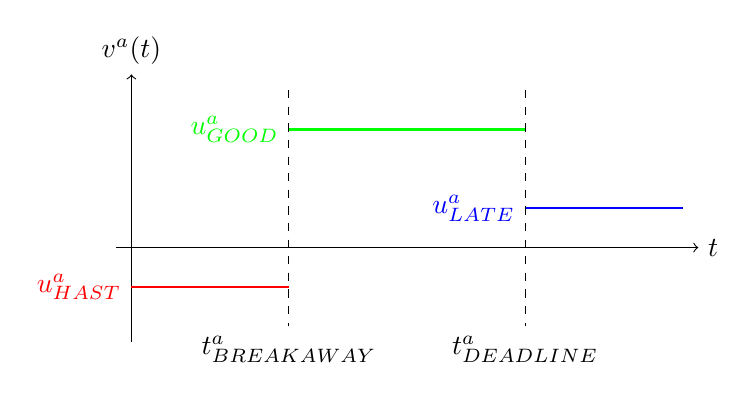
\begin{tikzpicture}[domain=0:7,scale=1]%,background rectangle/.style={fill=blue!20}, show background rectangle]
			\draw[->] (-0.2,0) -- (7.2,0) node[right] {$t$};
			\draw[->] (0,-1.2) -- (0,2.2) node[above] {$v^a(t)$};
			\draw[red, thick] (2, -0.5) -- (0, -0.5) node[left] {$u^a_{HAST}$};
			\draw[green, thick] (5, 1.5) -- (2, 1.5) node[left] {$u^a_{GOOD}$};
			\draw[blue, thick] (7, 0.5) -- (5, 0.5) node[left] {$u^a_{LATE}$};
			\draw[dashed] (2, 2) -- (2, -1) node[below] {$t^a_{BREAKAWAY}$};
			\draw[dashed] (5, 2) -- (5, -1) node[below] {$t^a_{DEADLINE}$};
		\end{tikzpicture}
	\end{center}
\end{frame}

\subsection{Смешанные равновесия игры $\Gamma^3_n$}

\begin{frame}
	\frametitle{Игра $\Gamma^3_n$}
	\begin{itemize}
		\item $t_i^1 = t_i^2 = t_i^3 = 2, i = \overline{1,n}$
		\item $t^1_{DEADLINE} = t^2_{DEADLINE} = t^3_{DEADLINE} = 5$
		\item $t^1_{BREAKAWAY} = t^2_{BREAKAWAY} = t^3_{BREAKAWAY} = 3$
		\item $u^1_{LATE} = u^2_{LATE} = u^3_{LATE} = 2$
		\item $u^1_{GOOD} = u^2_{GOOD} = u^3_{GOOD} = 3$
		\item $u^1_{HAST} = u^2_{HAST} = u^3_{HAST} = 0$
	\end{itemize}
\end{frame}

\begin{frame}
	\frametitle{Равновесия по Нэшу игры $\Gamma^3_n$}
	\begin{block}{Лемма}
		Пусть $T \subseteq \{1, \ldots, n\}$ "--- произвольное непустое подмножество компьютеров. Тогда в игре $\Gamma^3_n$ набор одинаковых смешанных стратегий $s^1 = s^2 = s^3 = \left(\frac{[1 \in T]}{\left| T \right|}, \ldots, \frac{[n \in T]}{\left| T \right|}\right)$, где каждый игрок независимо и равновероятно выбирает одну из машин множества $T$, является равновесием по Нэшу.\footnote{Здесь и далее для упрощения и сокращения записи используется нотация <<скобка Айверсона>>: $[\textsc{true}] = 1, [\textsc{false}] = 0$.}
	\end{block}
	\begin{equation*}
		u^1(s) = u^2(s) = u^3(s) = \frac{6 \left| T \right| - 4}{\left| T \right|^2}
	\end{equation*}
\end{frame}

\begin{frame}
	\frametitle{Отсутствие других равновесий}
	\begin{block}{Лемма}
		В игре $\Gamma^3_n$ набор смешанных стратегий $s = (s^1, s^2, s^3)$ может быть равновесием по Нэшу только в том случае, когда $s^1 = s^2 = s^3$.
	\end{block}
	\begin{block}{Лемма}
		В игре $\Gamma^3_n$ набор одинаковых смешанных стратегий может быть равновесием по Нэшу только в том случае, когда все компьютеры, выбираемые с ненулевой вероятностью, выбираются с равными вероятностями.
	\end{block}
\end{frame}

\begin{frame}
	\frametitle{Достижимые вектора выплат}
	\begin{align*}
		\min_{\emptyset \subset T \subseteq \{1,\ldots,n\}} \frac{6 \left| T \right| - 4}{\left| T \right|^2} &= \frac{6 n - 4}{n^2};\\
		\max_{\emptyset \subset T \subseteq \{1,\ldots,n\}} \frac{6 \left| T \right| - 4}{\left| T \right|^2} &= 2.
	\end{align*}
	Выпуклая оболочка множества достижимых векторов выплат представляет собой отрезок, соединяющий точки $(2, 2, 2)$ и $(\frac{6 n - 4}{n^2}, \frac{6 n - 4}{n^2}, \frac{6 n - 4}{n^2})$.
\end{frame}

%\begin{frame}
%    \frametitle{Разделяющие линии}
%    \begin{minipage}[c]{0.47\linewidth}
%        \center{\includegraphics[width=1\linewidth]{latex}}
%        \bigskip
%        \hrule{}
%        \bigskip
%        \textbf{Составная \\ подпись 1}
%    \end{minipage}
%    \hfill
%    \vrule{}
%    \hfill
%    \begin{minipage}[c]{0.47\linewidth}
%        \flushright
%        \textbf{Составная \\ подпись 2}
%        \center{\includegraphics[width=1\linewidth]{knuth2}}
%    \end{minipage}
%\end{frame}

\subsection{Равновесия игры $\Gamma^3_n$ в пространстве заговоров}

\begin{frame}
	\frametitle{Пространство заговоров $\mathfrak{A} = \{\{1,2\}\}$}
	\begin{itemize}
		\item $\Omega = \left[0, 1\right)$,
		\item $\mathfrak{I}^1 = \mathfrak{I}^2 = \sigma(\{\left[ 0, p \right) \mid 0 < p \leq 1 \})$,
		\item $\mathfrak{I}^3 = \{\emptyset, \Omega\}$.
	\end{itemize}
\end{frame}

\begin{frame}
	\frametitle{Дополнительные решения игры $\Gamma^3_n | \{\{1,2\}\}$}
	\begin{align*}
		\mathbf{s}^1(\omega) = \mathbf{s}^2(\omega) &= ([\zeta(\omega) = 1], \ldots, [\zeta(\omega) = n]); \\ \mathbf{s}^3(\omega) &= \left(\frac{[1 \in T]}{\left| T \right|}, \ldots, \frac{[n \in T]}{\left| T \right|}\right),
	\end{align*}
	где общая для игроков 1 и 2 функция $\zeta : \left[0, 1\right) \rightarrow T$ определяет разбиение рулетки на $\left| T \right|$ равных секторов. Выплаты в этом наборе уже не симметричны:
	\begin{align*}
		u^1(\mathbf{s}) = u^2(\mathbf{s}) &= \frac{\left| T \right| - 1}{\left| T \right|} u^a_{GOOD} + \frac{1}{\left| T \right|} u^a_{LATE} = \frac{3 \left| T \right| - 1}{\left| T \right|};\\
		u^3(\mathbf{s}) &= \frac{\left| T \right| - 1}{\left| T \right|} u^a_{HAST} + \frac{1}{\left| T \right|} u^a_{LATE} = \frac{2}{\left| T \right|}.
	\end{align*}
\end{frame}

\subsection{Коллективная рациональность решений}

\begin{frame}
	\frametitle{Выплаты в равновесиях игр $\Gamma^3_n$ и $\Gamma^3_n | \{\{1,2\}\}$}
	\begin{center}
		\begin{tikzpicture}[domain=0:7,scale=1]%,background rectangle/.style={fill=blue!20}, show background rectangle]
			\draw[->] (-0.2,0) -- (7.2,0) node[right] {$\left| T \right|$};
			\draw[->] (0,-0.2) -- (0,3.2) node[above] {$u^a(s)$};
			\foreach \x in {1,...,6} {
				\draw [shift={(\x,0)}, color=black] (0pt,2pt) -- (0pt,-2pt) node [below] {\footnotesize $\x$};
				\node [draw, circle, inner sep=1pt, fill, color=blue] at (\x, {(6 * \x - 4) / (\x * \x)}) {};
				\only<2>{
					\node [draw, circle, inner sep=1pt, fill, color=green] at (\x, {(3 * \x - 1) / \x}) {};
					\node [draw, circle, inner sep=1pt, fill, color=red] at (\x, 2 / \x) {};
				}
			}
			\only<2>{\node [draw, circle, inner sep=1pt, fill] at (1, 2) {};}
			\node [right=6pt, color=blue] at (6, {(6 * 6 - 4) / (6 * 6)}) {$u^{1,2,3}(s)$};
			\only<2>{
				\node [right=6pt, color=green] at (6, {(3 * 6 - 1) / 6}) {$u^{1,2}(\mathbf{s})$};
				\node [right=6pt, color=red] at (6,  2 / 6) {$u^3(\mathbf{s})$};
			}
			\foreach \y in {1,2,3} \draw [shift={(0,\y)}, color=black] (2pt,0pt) -- (-2pt,0pt) node[left] {\footnotesize $\y$};
		\end{tikzpicture}
	\end{center}
\end{frame}

\begin{frame}
	\frametitle{Структурная согласованность равновесий}
	\begin{block}{Определение}
		В игре с заговорами $\Gamma | \mathfrak{A}$ равновесие по Нэшу $\mathbf{s}$ называется структурно согласованным, если для всех заговоров $A_* \in \mathfrak{A}$ отсутствуют приемлемые отклонения от ситуации $\mathbf{s}$.
	\end{block}
	\begin{block}{Определение}
		В игре с заговорами $\Gamma | \mathfrak{A}$ ситуацию $\mathbf{s}_* \neq \mathbf{s}$ назовём отклонением от $\mathbf{s}$, приемлемым для заговора $A_* \in \mathfrak{A}$, если
		\begin{itemize}
			\item $\forall a \notin A_* \quad \mathbf{s}^a = \mathbf{s}_*^a$;
			\item $\forall a \in A_* \quad u^a(\mathbf{s}_*) \geq u^a(\mathbf{s})$;
			\item $\forall a : \mathbf{s}^a \neq \mathbf{s}_*^a \quad u^a(\mathbf{s}_*) > u^a(\mathbf{s})$.
		\end{itemize}
	\end{block}
\end{frame}

\begin{frame}
	\frametitle{Структурно согласованные равновесия игры $\Gamma^3_n | \mathfrak{A}$}
	В игре с заговорами $\Gamma^3_n | \mathfrak{A}$ структурно согласованное равновесие Нэша существует при любых $n$ и $\mathfrak{A}$. При невырожденном $\mathfrak{A}$, каждому заговору из двух участников соответствует единственное такое равновесие, где ожидаемый выигрыш обоих заговорщиков составляет $\frac{3 n - 1}{n}$, а аутсайдера "--- $\frac{2}{n}$.
\end{frame}

\subsection{Немонотонная отдача в других конфликтах планирования}

\begin{frame}[allowframebreaks]
	\frametitle{Немонотонная отдача в конкуренции стандартов}
	Пусть $m$ компаний готовятся выйти на рынок с предложениями высокотехнологичного товара, и перед ними встаёт выбор между $n$ различными открытыми стандартами на один и тот же его важный аспект. К примеру, это могут быть разнообразные промышленные роботы и стандарты их интеграции в <<умный>> цех. Когда компания $a \in \{1, \ldots, m\}$ выходит на рынок стандарта $i \in \{1, \ldots, n\}$, она тем самым осуществляет вклад в его развитие, характеризующийся векторной константой $t_i^a \in \mathbb{R}_{\ge 0} \times \ldots \times \mathbb{R}_{\ge 0}$, компоненты которой соответствуют отдельным независимым аспектам (например, функциям, для исполнения которых приобретаются роботы). Если в ситуации $s$ одним стандартом $i$ пользуются несколько компаний, то простым суммированием их вкладов можно посчитать общий индекс развития $t_i(s) = [s^1 = i] t_i^1 + \ldots + [s^m = i] t_i^m$. На ожидаемый доход от инвестиций в каждый из стандартов существенным образом влияют два дисконтирующих фактора: сетевой эффект и насыщение рынка.
	
	\framebreak
	
	Под сетевым эффектом мы понимаем зависимость покупательского энтузиазма от общего индекса развития стандарта "--- функция $0 \le \alpha^a(t) \le 1$ характеризует долю покупателей, готовых приобретать роботов компании $a$, выполненных по стандарту с общим индексом развития $t$. Более развитый стандарт всегда привлекает больше потребителей, так что функции $\alpha^a(t)$ монотонно неубывающие, т.е. $\alpha^a(t) \le \alpha^a(t + \Delta), \forall t, \Delta \succeq (0, \ldots, 0)$.
	
	\framebreak
	
	Насыщение рынка, с другой стороны, подразумевает ограниченность спроса "--- при избытке инвестиций в любой из стандартов, платёжеспособности покупателей перестаёт хватать на всех, цены приходится снижать, а с ними падают и доходы. Соответственно, ещё одна функция $0 \le \beta^a(t) \le 1$ характеризует, какой долей прибыли придётся ограничиться компании $a$ для сохранения конкурентоспособности своих роботов на рынке стандарта с общим индексом развития $t$. Эта функция, по понятным причинам, монотонно невозрастающая, т.е. $\beta^a(t) \ge \beta^a(t + \Delta), \forall t, \Delta \succeq (0, \ldots, 0)$. Целью компании $a$ при выборе стратегии $s^a$ является максимизация комбинации дисконтирующих факторов $u^a(s) = \alpha^a(t_{s^a}(s)) \beta^a(t_{s^a}(s))$.
\end{frame}

\begin{frame}[allowframebreaks]
	\frametitle{Немонотонная отдача в представительной демократии}
	Можно представить и политическую интерпретацию этой же игры. Пусть в некий коллегиальный выборный орган пытаются избираться $n$ кандидатов (самостоятельно, без партийных списков), а $m$ эффективных менеджеров выбирают, за кого из них развернуть агитацию в подведомственных учреждениях. Когда олигарх $a$ принимает решение о поддержке кандидата $i$, тем самым он вносит вклад в его популярность, характеризующийся векторной константой $t_i^a \in \mathbb{R}_{\ge 0} \times \ldots \times \mathbb{R}_{\ge 0}$, компоненты которой соответствуют электорально значимым демографическим группам. Если в ситуации $s$ кандидата $i$ поддерживают несколько олигархов, то простым суммированием их вкладов можно получить общий индекс популярности кандидата $t_i(s) = [s^1 = i] t_i^1 + \ldots + [s^m = i] t_i^m$. На ожидаемую выгоду от поддержки того или иного кандидата влияют два дисконтирующих фактора: политическое влияние и готовность к сотрудничеству.
	
	\framebreak
	
	Политическое влияние кандидата в вопросах, интересующих поддержавшего его олигарха, очевидно, растёт вместе с общим индексом его популярности, что выражается функцией $0 \le \alpha^a(t) \le \alpha^a(t + \Delta) \le 1, \forall t, \Delta \succeq (0, \ldots, 0)$. Готовность же кандидата к сотрудничеству с каждым из своих сторонников, наоборот, падает с ростом его суммарной популярности, что выражается функцией $1 \ge \beta^a(t) \ge \beta^a(t + \Delta) \ge 0, \forall t, \Delta \succeq (0, \ldots, 0)$. Целью олигарха $a$ при выборе стратегии $s^a$ является максимизация комбинации дисконтирующих факторов $u^a(s) = \alpha^a(t_{s^a}(s)) \beta^a(t_{s^a}(s))$.
\end{frame}

\begin{frame}
	\frametitle{Матричная игра в нормальной форме}
	\begin{equation*}
		\Gamma = \langle A, S^a, u^a(s), a \in A \rangle;
	\end{equation*}
	\begin{equation*}
		A = \{1, \ldots, m\}, S^1 = \ldots = S^m = \{1, \ldots, n\};
	\end{equation*}
	\begin{equation*}
		u^a(s) = \alpha^a(t_{s^a}(s)) \beta^a(t_{s^a}(s)), a = \overline{1,m};
	\end{equation*}
	\begin{equation*}
		\alpha^a, \beta^a : \mathbb{R}_{\ge 0} \times \ldots \times \mathbb{R}_{\ge 0} \rightarrow [0, 1];
	\end{equation*}
	\begin{equation*}
		0 \le \alpha^a(t) \le \alpha^a(t + \Delta) \le 1, \forall t, \Delta \succeq (0, \ldots, 0);
	\end{equation*}
	\begin{equation*}
		1 \ge \beta^a(t) \ge \beta^a(t + \Delta) \ge 0, \forall t, \Delta \succeq (0, \ldots, 0);
	\end{equation*}
	\begin{equation*}
		t_i(s) = [s^1 = i] t_i^1 + \ldots + [s^m = i] t_i^m, i = \overline{1,n}.
	\end{equation*}
\end{frame}

\begin{frame}
	\frametitle{Многомерная квазивогнутость}
	Во избежание переусложнения ограничимся случаем квазивогнутых функций отдачи, естественным образом обобщив это понятие на многомерные области определения. Для начала обозначим символом $T^a_{\nearrow}$ множество всех таких $t$, что $t_* \prec t \Rightarrow v^a(t_*) \le v^a(t) \wedge t_* \in T^a_{\nearrow}$. Аналогично, символом $T^a_{\searrow}$ обозначим множество всех таких $t$, что $t_* \succ t \Rightarrow v^a(t_*) \le v^a(t) \wedge t_* \in T^a_{\searrow}$. Это будут области непрерывного неубывания и невозрастания $v^a(t)$ соответственно. Если эти два множества покрывают всю область определения, т.е. $T^a_{\nearrow} \cup T^a_{\searrow} = \mathbb{R}_{\ge 0} \times \ldots \times \mathbb{R}_{\ge 0}$, то функция $v^a(t)$ квазивогнута. Для подобных функций также можно обозначить <<гребень>> $T^a_{\sim} = T^a_{\nearrow} \cap T^a_{\searrow}$, в одномерном случае соответствующий максимуму.
\end{frame}

\begin{frame}
	\frametitle{Смысл структурной согласованности равновесий}
	Интересны с точки зрения теории заговоров ситуации, когда группа игроков может достичь гребня своих функций отдачи, только выбирая стратегию совместно, причём присоединение дополнительных игроков уже выводит результат за гребень. В подобных случаях можно ожидать, что такая группа захочет координировать свои действия втайне от остальных. По сути формализм структурно согласованного равновесия в играх с заговорами является не какой-то сложной экономической концепцией, а всего лишь воплощением интуитивного принципа, применявшегося, вероятно, ещё в дописьменную эпоху. Вполне возможно, что накой-нибудь охотник, заметив раненного мамонта при обходе племенных угодий, рассудил: <<В одиночку я его, пожалуй, не завалю, но и племя всё звать смысла нет. Шепну-ка я лучше на ушко паре друзей "--- это ж сколько почёта и славы будет, втроём столько мяса добыть.>> С похожего рассуждения и могла начаться мировая история заговоров.
\end{frame}

\section{Вычислительная сложность стратегий в повторяющихся играх}
\begin{frame}[plain, noframenumbering]
    \begin{center}
        \Huge
        Вычислительная сложность стратегий в повторяющихся играх с дисконтированием
    \end{center}
\end{frame}

\subsection{<<Народная>> теорема в пространствах заговоров}

\begin{frame}
	\frametitle{Резервные выигрыши и точка минимакса}
	\begin{block}{Обычный}
		\begin{equation*}
			u^a_* = \min_{s \in \overline{S}_a} u^a(s), \overline{S}_a = \{\overline{s} \in S \mid \overline{s}^a \in \arg\max_{s^a \in S^a} u^a(\overline{s} | s^a)\}
		\end{equation*}
	\end{block}
	\begin{block}{Равновесный}
		\begin{equation*}
			\tilde{u}^a_* = \min_{s \in \tilde{S}} u^a(s), \text{где $\tilde{S}$ "--- множество равновесных по Нэшу наборов}
		\end{equation*}
	\end{block}
	Вектора $u_* = (u^1_*, \ldots, u^m_*)$ и $\tilde{u}_* = (\tilde{u}^1_*, \ldots, \tilde{u}^m_*)$, составленные из резервных выигрышей каждого игрока, называются точками обычного и равновесного минимакса соответственно.
\end{frame}

\begin{frame}
	\frametitle{<<Народная>> теорема для пространств заговоров}
	\begin{block}{Теорема}
		Пусть $\Gamma = \langle A, S^a, u^a(s), a \in A \rangle$ "--- игра в нормальной форме с конечным множеством исходов, $V$ "--- выпуклая оболочка множества платёжных векторов её матрицы, а $\mathfrak{A} \subseteq 2^A$ "--- произвольное пространство заговоров. Если вектор выплат $v \in V$ строго доминирует точку минимакса игры $\Gamma | \mathfrak{A}$, то найдётся такой коэффициент дисконтирования $0 < \delta < 1$, что в бесконечно повторяющейся игре $\Gamma | \mathfrak{A}$ будет существовать равновесие Нэша с выплатами, сходящимися к $v$. Если же вектор $v$ доминирует ещё и точку равновесного минимакса той же игры, то в бесконечно повторяющейся игре с достаточно большим коэффициентом дисконтирования будет существовать совершенное подыгровое равновесие с выплатами, сходящимися к $v$.
	\end{block}
\end{frame}

%\begin{frame}
%    \frametitle{Формулы}
%    \[
%    \left\{
%    \begin{array}{rl}
%        \dot x = & \sigma (y-x)  \\
%        \dot y = & x (r - z) - y \\
%        \dot z = & xy - bz
%    \end{array}
%    \right.
%    \]
%\end{frame}
%
%\begin{frame}
%    \frametitle{amsmath}
%    \centering
%    \begin{minipage}[t]{0.5\linewidth}
%        \begin{multline*}
%            y = 1 x^1 + 2 x^2 + 3 x^3 + \\ + 4 x^4 + 5 x^5 + \dots
%        \end{multline*}
%    \end{minipage}
%\end{frame}
%
%\begin{frame}[allowframebreaks]
%    \frametitle{Уравнения Максвелла}
%    \centering{
%        \small
%        \def\arraystretch{1.8}%
%        \begin{tabular}{ll}
%            \toprule
%            Интегральная форма                                                                                                                                            & Дифференциальная форма                                                          \\ \midrule
%            \(Q_e(t) = \displaystyle\oiint_S \vec D(t) \cdot d\vec{s} = \displaystyle\iiint_V \rho_v(t) dv\)                                                              & \(\nabla \cdot \vec D(t) = \rho_v(t)\)                                          \\
%            \(\displaystyle\oiint_S \vec B(t) \cdot d\vec{s} = 0\)                                                                                                        & \(\nabla \cdot \vec B(t) = 0\)                                                  \\
%            \(V_{emf}(t) = \displaystyle\oint_L \vec E(t) \cdot d\vec{l}\) = \(- \displaystyle\iint_S \left[\frac{\partial\vec{B}(t)}{\partial t}\right] \cdot d\vec{s}\) & \(\nabla \times \vec E(t) = - \frac{\partial\vec{B}(t)}{\partial t}\)           \\
%            \(I(t) = \displaystyle\oint_L \vec H(t) \cdot d\vec{l} = \displaystyle\iint_S \left[\vec J(t) + \frac{\partial\vec{D}(t)}{\partial t}\right] \cdot d\vec{s}\) & \(\nabla \times \vec H(t) = \vec J(t) + \frac{\partial\vec{D}(t)}{\partial t}\) \\ \midrule
%            \(\displaystyle\oiint_S \vec J \cdot d\vec{s} = -\frac{\partial Q_e}{\partial t}\)                                                                            & \(\nabla \cdot \vec J = - \frac{\partial \rho_v}{\partial t}\)                  \\
%            \bottomrule
%            \multicolumn{2}{c}{\(\vec D(t) = \left[\varepsilon(t)\right] * \vec E(t)\)}                                                                                                                                                                     \\
%            \multicolumn{2}{c}{\(\vec B(t) = \left[\mu(t)\right] * \vec H(t)\)}                                                                                                                                                                             \\
%        \end{tabular}
%    }
%    \framebreak
%
%    \hspace{0.05\linewidth}
%    \centering{
%        \small
%        \def\arraystretch{1.8}%
%        \begin{tabular}{ll}
%            \toprule
%            Интегральная форма                                                                                                                & Дифференциальная форма                               \\ \midrule
%            \(Q_e = \displaystyle\oiint_S \vec D \cdot d\vec{s} = \displaystyle\iiint_V \rho_v dv\)                                           & \(\nabla \cdot \vec D = \rho_v\)                     \\
%            \(\displaystyle\oiint_S \vec B \cdot d\vec{s} = 0\)                                                                               & \(\nabla \cdot \vec B = 0\)                          \\
%            \(V_{emf} = \displaystyle\oint_L \vec E \cdot d\vec{l}\) = \(- \displaystyle\iint_S \left[j \omega \vec B\right] \cdot d\vec{s}\) & \(\nabla \times \vec E = - j \omega \vec B\)         \\
%            \(I = \displaystyle\oint_L \vec H \cdot d\vec{l} = \displaystyle\iint_S \left[\vec J + j \omega \vec D\right] \cdot d\vec{s}\)    & \(\nabla \times \vec H = \vec J + j \omega \vec{D}\) \\ \midrule
%            \(\displaystyle\oiint_S \vec J \cdot d\vec{s} = - j \omega Q_e\)                                                                  & \(\nabla \cdot \vec J = - j \omega \rho_v\)          \\
%            \bottomrule
%            \multicolumn{2}{c}{\(\vec D(t) = \left[\varepsilon\right] \vec E(t)\)}                                                                                                                   \\
%            \multicolumn{2}{c}{\(\vec B(t) = \left[\mu\right] \vec H(t)\)}                                                                                                                           \\
%        \end{tabular}
%    }
%\end{frame}

\subsection{Повторяющийся трёхсторонний чёт-нечет}

\begin{frame}
	\frametitle{Пример повторяющейся игры}
	\begin{table} [htbp]
		\centering
		\begin{threeparttable}
			\caption{Трёхсторонний чёт"~нечет}
			%			\label{tab:coin3}
			\begin{tabular}{ |c|c|c|c|c| }
				\cline{1-2} \cline{4-5}
				\rule[-7pt]{0pt}{2em}$4, 4, 4$ &
				\rule[-7pt]{0pt}{2em}$6, 0, 6$ & \qquad\qquad\qquad &
				\rule[-7pt]{0pt}{2em}$6, 6, 0$ &
				\rule[-7pt]{0pt}{2em}$0, 6, 6$ \\
				\cline{1-2} \cline{4-5}
				\rule[-7pt]{0pt}{2em}$0, 6, 6$ &
				\rule[-7pt]{0pt}{2em}$6, 6, 0$ & \qquad\qquad\qquad &
				\rule[-7pt]{0pt}{2em}$6, 0, 6$ &
				\rule[-7pt]{0pt}{2em}$4, 4, 4$ \\
				\cline{1-2} \cline{4-5}
			\end{tabular}
		\end{threeparttable}
	\end{table}
	\begin{block}{Без информационной асимметрии}
		Резервные выигрыши равны $u^1_* = u^2_* = u^3_* = 4$. Множество решений не пополняется.
	\end{block}
	\begin{block}{В пространстве заговоров $\mathfrak{A}$}
		Каждый двухместный заговор снижает резервный выигрыш аутсайдера до $2$. Таким образом, $\forall a \in \{1, 2, 3\}$:
		\begin{equation*}
			u^a_* = \begin{cases}
				4, & \{1, 2, 3\} \setminus \{a\} \notin \mathfrak{A};\\
				2, & \{1, 2, 3\} \setminus \{a\} \in \mathfrak{A}.
			\end{cases}
		\end{equation*}
	\end{block}
\end{frame}

\begin{frame}
	\frametitle{Новые точки равновесия}
	В одиночном розыгрыше трёхстороннего чёт"~нечета с любым $\mathfrak{A}$ нет точек равновесия, в которых выигрыш какого-либо игрока превосходит $5$. Однако, при бесконечном повторении с коэффициентом дисконтирования $\delta \ge \frac{2}{3}$ пространство заговоров $\{\{1, 3\}, \{2, 3\}\}$, например, позволяет построить решение с выплатами $(3, 3, 6)$. Игроки договариваются о том, что
	\begin{itemize}
		\item игрок 1 всегда выбирает орла;
		\item игрок 2 всегда выбирает решку;
		\item игрок 3 выбирает между орлом и решкой случайно и равновероятно;
		\item если кто-либо из пары игроков 1 и 2 отклоняется от предписанной стратегии, то другой вместе с игроком 3 используют в качестве наказания коррелированные стратегии с выплатами $(2, 5, 5)$ или $(5, 2, 5)$ соответственно.
	\end{itemize}
\end{frame}

%\begin{frame}
%    \frametitle{Таблица}
%    \centering
%    \begin{tabular}{|l|l|}
%        \hline
%        \textbf{Заголовок 1} & \textbf{Заголовок 2} \\
%        \hline
%        Сумма                & \(b+a\)              \\
%        \hline
%        Разность             & \(a-b\)              \\
%        \hline
%        Произведение         & \(a*b\)              \\
%        \hline
%    \end{tabular}
%\end{frame}
%
%\begin{frame}
%    \frametitle{Другая таблица}
%    \centering
%    \begin{tabular}{lc}
%        \toprule
%        \multicolumn{1}{c}{\textbf{Заголовок 1}} & \textbf{Заголовок 2} \\ \midrule
%        Сумма                                    & \(b+a\)              \\
%        Разность                                 & \(a-b\)              \\
%        Произведение                             & \(a*b\)              \\
%        \bottomrule
%    \end{tabular}
%\end{frame}


\subsection{Модель повторяющихся игр с учётом стоимости вычислений}

\begin{frame}
	\frametitle{Схема взаимодействий в модели}
	\begin{block}{Повторяющаяся игра с учётом стоимости вычислений}
		\begin{center}			
			\begin{tikzpicture}[scale=1.4]
				\node[circle,draw] (game1) at (1, 0) {$\Gamma$};
				\node[circle,draw] (game2) at (3, 0) {$\Gamma$};
				\node[circle,draw] (game3) at (5, 0) {$\Gamma$};
				\node[rectangle,draw] (calc11) at (0,  1) {$M^1$};
				\node[rectangle,draw] (calc12) at (2,  1) {$M^1$};
				\node[rectangle,draw] (calc13) at (4,  1) {$M^1$};
				\node[] (calc1i) at (6, 1) {$\cdots$};
				\node[rectangle,draw] (calc21) at (0, -1) {$M^2$};
				\node[rectangle,draw] (calc22) at (2, -1) {$M^2$};
				\node[rectangle,draw] (calc23) at (4, -1) {$M^2$};
				\node[] (calc2i) at (6, -1) {$\cdots$};
				\draw [->,thick,decorate,decoration={snake,post length=1mm}] (calc11) -- (game1) node[midway,sloped,below] {$s^1_0$};
				\draw [->,thick,decorate,decoration={snake,post length=1mm}] (calc21) -- (game1) node[midway,sloped,above] {$s^2_0$};
				\draw [->,thick,decorate,decoration={snake,post length=1mm}] (calc12) -- (game2) node[midway,sloped,below] {$s^1_1$};
				\draw [->,thick,decorate,decoration={snake,post length=1mm}] (calc22) -- (game2) node[midway,sloped,above] {$s^2_1$};
				\draw [->,thick,decorate,decoration={snake,post length=1mm}] (calc13) -- (game3) node[midway,sloped,below] {$s^1_2$};
				\draw [->,thick,decorate,decoration={snake,post length=1mm}] (calc23) -- (game3) node[midway,sloped,above] {$s^2_2$};
				\draw [->,thick,decorate,decoration={snake,post length=1mm}] (game1) -- (calc12) node[midway,sloped,below] {$s_0$};
				\draw [->,thick,decorate,decoration={snake,post length=1mm}] (game1) -- (calc22) node[midway,sloped,above] {$s_0$};
				\draw [->,thick,decorate,decoration={snake,post length=1mm}] (game2) -- (calc13) node[midway,sloped,below] {$s_1$};
				\draw [->,thick,decorate,decoration={snake,post length=1mm}] (game2) -- (calc23) node[midway,sloped,above] {$s_1$};
				\draw [->,thick,decorate,decoration={snake,post length=1mm}] (game3) -- (calc1i) node[midway,sloped,below] {$s_2$};
				\draw [->,thick,decorate,decoration={snake,post length=1mm}] (game3) -- (calc2i) node[midway,sloped,above] {$s_2$};
				\node[diamond,draw] (sum1) at (-1, 2) {$\Sigma^1$};
				\node[] (sum10) at (0,  2) [label=$-\mathfrak{w}^1_0$] {};
				\node[] (sum11) at (1,  2) [label=$+u^1(s_0)$] {};
				\node[] (sum12) at (2,  2) [label=$-\delta \mathfrak{w}^1_1$] {};
				\node[] (sum13) at (3,  2) [label=$+\delta u^1(s_1)$] {};
				\node[] (sum14) at (4,  2) [label=$-\delta^2 \mathfrak{w}^1_2$] {};
				\node[] (sum15) at (5,  2) [label=$+\delta^2 u^1(s_2)$] {};
				\node[] (sum1i) at (6,  2) {$\cdots$};
				\node[diamond,draw] (sum2) at (-1, -2) {$\Sigma^2$};
				\node[] (sum20) at (0, -2) [label=below:$-\mathfrak{w}^2_0$] {};
				\node[] (sum21) at (1, -2) [label=below:$+u^2(s_0)$] {};
				\node[] (sum22) at (2, -2) [label=below:$-\delta \mathfrak{w}^2_1$] {};
				\node[] (sum23) at (3, -2) [label=below:$+\delta u^2(s_1)$] {};
				\node[] (sum24) at (4, -2) [label=below:$-\delta^2 \mathfrak{w}^2_2$] {};
				\node[] (sum25) at (5, -2) [label=below:$+\delta^2 u^2(s_2)$] {};
				\node[] (sum2i) at (6, -2) {$\cdots$};
				\draw [->,thick] (sum1i) -- (sum1);
				\draw [->,thick] (calc11) -- (sum10);
				\draw [->,thick] (game1) -- (sum11);
				\draw [->,thick] (calc12) -- (sum12);
				\draw [->,thick] (game2) -- (sum13);
				\draw [->,thick] (calc13) -- (sum14);
				\draw [->,thick] (game3) -- (sum15);
				\draw [->,thick] (sum2i) -- (sum2);
				\draw [->,thick] (calc21) -- (sum20);
				\draw [->,thick] (game1) -- (sum21);
				\draw [->,thick] (calc22) -- (sum22);
				\draw [->,thick] (game2) -- (sum23);
				\draw [->,thick] (calc23) -- (sum24);
				\draw [->,thick] (game3) -- (sum25);
				\fill [white] (1,  1) circle (2pt);
				\fill [white] (3,  1) circle (2pt);
				\fill [white] (5,  1) circle (2pt);
				\fill [white] (1, -1) circle (2pt);
				\fill [white] (3, -1) circle (2pt);
				\fill [white] (5, -1) circle (2pt);
				\draw [->,double,thick] (-1,  1) -- (calc11) node[midway,above] {$\psi^1_0$};
				\draw [->,double,thick] (calc11) -- (calc12) node[near end,above] {$\psi^1_1$};
				\draw [->,double,thick] (calc12) -- (calc13) node[near end,above] {$\psi^1_2$};
				\draw [->,double,thick] (calc13) -- (calc1i) node[near end,above] {$\psi^1_3$};
				\draw [->,double,thick] (-1, -1) -- (calc21) node[midway,below] {$\psi^2_0$};
				\draw [->,double,thick] (calc21) -- (calc22) node[near end,below] {$\psi^2_1$};
				\draw [->,double,thick] (calc22) -- (calc23) node[near end,below] {$\psi^2_2$};
				\draw [->,double,thick] (calc23) -- (calc2i) node[near end,below] {$\psi^2_3$};
			\end{tikzpicture}
		\end{center}
	\end{block}
\end{frame}

\begin{frame}
	\frametitle{Функции полезности с учётом стоимости вычислений}
	Поскольку мы говорим о конфликтах рациональных агентов, имеет смысл рассматривать только универсальные алгоритмы $M^a$, позволяющие закодировать любой набор вычислимых стратегий повторяющейся игры в начальных состояниях памяти $\psi^a_0$. Нотация $M^a[g]$ будет обозначать среднюю стоимость вычисления произвольной функции $g$ при её оптимальной реализации посредством $M^a$. Кроме того, если обозначить символом $\mathfrak{s}$ набор стратегий повторяющейся игры с дисконтированием, то нотация $M^a[\mathfrak{s}]$ подходит для обозначения стоимости полного объёма вычислений, необходимых игроку $a$ для выбора каждого хода с учётом того же коэффициента $\delta$. Таким образом, в повторяющейся игре с учётом стоимости вычислений каждый игрок $a$ оптимизирует не просто $u^a(\mathfrak{s})$, но
	\begin{equation*}
		\hat{u}^a(\mathfrak{s}) = u^a(\mathfrak{s}) - M^a[\mathfrak{s}].	
	\end{equation*}
\end{frame}

%\begin{frame}
%    \frametitle{Большой многоуровневый список}
%    \begin{itemize}
%        \item \textbf{Пункт 1}
%              \begin{itemize}
%                  \itemi Подпункт 1-1
%                  \itemi Подпункт 1-2
%              \end{itemize}
%        \item \textbf{Пункт 2}
%              \begin{itemize}
%                  \itemi Подпункт 2-1
%              \end{itemize}
%        \item \textbf{Пункт 3}
%              \begin{itemize}
%                  \itemi Подпункт 3-1
%                  \itemi Подпункт 3-2
%              \end{itemize}
%        \item \textbf{Пункт 4}
%              \begin{itemize}
%                  \itemi Подпункт 4-1
%              \end{itemize}
%        \item \textbf{Пункт 5}
%              \begin{itemize}
%                  \itemi Подпункт 5-1
%                  \itemi Подпункт 5-2
%                  \itemi Подпункт 5-3
%              \end{itemize}
%    \end{itemize}
%\end{frame}
%
%\begin{frame}
%    \frametitle{Четыре изображения}
%    \centering
%    \includegraphics[width=0.35\linewidth,angle=35]{latex}
%    \includegraphics[width=0.35\linewidth,angle=135]{latex}\\
%    \includegraphics[width=0.35\linewidth,angle=15]{latex}
%    \includegraphics[width=0.35\linewidth,angle=-15]{latex}
%\end{frame}

\subsection{Криптографическое согласование стратегий}

\begin{frame}[allowframebreaks]
	\frametitle{Общая схема протокола DH}
	Пусть имеется семейство биекций $f_n: \mathbb{N}_{<2^n} \leftrightarrow \mathbb{N}_{<2^n}, n \in \mathbb{N}$, обладающих свойством односторонности, т.е. для любого универсального вычислителя $M^*$ одновременно выполняется $M^*[f_n] \in o(2^n)$ (стоимость вычисления самой функции растёт с ростом $n$ полиномиально) и $M^*[f_n^{-1}] \in \Theta(2^n)$ (стоимость вычисления обратной функции растёт с ростом $n$ экспоненциально). Кроме этого, пусть имеется семейство двухместных функций $h_n : \mathbb{N}_{<2^n} \times \mathbb{N}_{<2^n} \rightarrow \mathbb{N}_{<2^n}$ таких, что
	\begin{itemize}
		\item $\forall x, y \in \mathbb{N}_{<2^n}, h_n(f_n(x), y) = h_n(x, f_n(y))$;
		\item $\forall x, y, z \in \mathbb{N}_{<2^n}, h_n(h_n(x, y), z) = h_n(x, h_n(y, z))$;
		\item $h_n(x_1, y_1) = h_n(x_2, y_2) \Rightarrow x_1 = x_2 \cap y_1 = y_2 \cup x_1 \neq x_2 \cap y_1 \neq y_2$.;
		\item $M^*[h_n] \in o(2^n)$.
	\end{itemize}
	\framebreak
	Алиса выбирает случайное натуральное число $0 \le x < 2^n$, выполняющее роль её закрытого ключа, и вычисляет $X = f_n(x)$, выполняющее роль её открытого ключа. На другом конце Боб аналогичным образом генерирует пару ключей $y$ и $Y = f_n(y)$. Алиса и Боб обмениваются открытыми ключами через прослушиваемый Кэрол канал связи. Теперь Алиса, зная свой закрытый ключ $x$ и открытый ключ Боба $Y$, может вычислить $h_n(x, Y)$, а Боб, соответственно, $h_n(X, y)$. В силу свойств функции $h_n$, вычисленные ими значения можно считать искомым общим секретным ключом $K = h_n(x, Y) = h_n(X, y)$. При этом для Кэрол, знающей только открытые ключи $X$ и $Y$, вычисление общего секретного ключа требует вычисления либо $f_n^{-1}(X)$, либо $f_n^{-1}(Y)$.
	
	\framebreak
	
	Благодаря разнице между асимптотической сложностью прямой и обратной функции всегда можно подобрать такое $n$, что стоимости вычисления $f_n$ и $h_n$ оказываются приемлемы, тогда как вычисление $f_n^{-1}$ "--- непозволительно дорогой процесс. Также заметим, что вследствие ассоциативности функции $h_n$ можно считать многоместными, и члены группы агентов любого размера могут комбинировать с их помощью общие секретные ключи, если каждый опубликовал свой открытый ключ "--- например, $K = h_n(x, Y, Z) = h_n(X, y, Z) = h_n(X, Y, z)$ для трёх сторон.
\end{frame}

\begin{frame}
	\frametitle{Криптографически стойкие генераторы псевдослучайных чисел}
	Вторым криптографическим примитивом, необходимым для стратегии наказания, является \emph{криптографически стойкий генератор псевдослучайных чисел}, далее называемый CSPRNG. Его можно представить в виде семейства функций $G_n : \mathbb{N}_{<2^n} \times \mathbb{N} \rightarrow \{0, 1\}$, первый аргумент которых называется зерном (или seed), а второй "--- позицией. Программа, вычисляющая для заданного $K \in \mathbb{N}_{<2^n}$ последовательные значения $G_n(K, i), i = 1, 2, \ldots$, должна совершать каждый шаг за полиномиальное от $n$ число операций. При этом генератор обязан проходить тест на следующий бит, т.е. не должно существовать полиномиально сложного от $n$ алгоритма, способного без знания $K$ по первым $i$ битам генерируемой последовательности угадать $G_n(K, i+1)$ с вероятностью, отличной от $\frac{1}{2}$.
\end{frame}

\begin{frame}[allowframebreaks]
	\frametitle{Криптографические стратегии}
	\begin{block}{$\mathfrak{s}^L_n$ <<рукопожатие влево>> ($\mathfrak{s}^R_n$ <<рукопожатие вправо>>)}
		\begin{enumerate}
			\item Выбрать случайное число $x \in \mathbb{N}_{<2^n}$.
			\item Вычислить $X = f_n(x)$ и представить в виде битовой последовательности $(X_i) \in \{0, 1\}^n$.
			\item Для каждого $i = 1 \ldots n$ совершить один ход игры, выбирая решку при $X_i = 1$ и орла в противном случае. Выбранную сидящим слева (справа) игроком стратегию (с тем же сопоставлением) запомнить в качестве очередного элемента битовой последовательности $(Y_i) \in \{0, 1\}^n$, соответствующей числу $Y \in \mathbb{N}_{<2^n}$.
			\item Вычислить $K = h_n(x, Y)$ (или $K = h_n(Y, x)$ соответственно).
			\item Все последующие ходы совершать, выбирая стратегию в соответствии с последовательно генерируемыми CSPRNG значениями $G_n(K, i), i = 1, 2, \ldots$.
		\end{enumerate}
	\end{block}
	
	\framebreak

	\begin{block}{$\mathfrak{s}^*_n$ <<взлом>>}
		\begin{enumerate}
			\item Первые $n$ ходов играть смешанную стратегию равновероятного выбора и запоминать ходы оппонентов для получения их открытых ключей $X$ и $Y$.
			\item Вычислить $K = h_n(f_n^{-1}(X), Y)$ или $K = h_n(X, f_n^{-1}(Y))$.
			\item Все последующие ходы совершать, выбирая стратегию в соответствии с последовательно генерируемыми CSPRNG значениями $G_n(K, i), i = 1, 2, \ldots$.
		\end{enumerate}
	\end{block}
	\begin{block}{$\mathfrak{s}^{\varnothing}$ <<пас>>}
		Игрок на каждой итерации просто выбирает между орлом и решкой случайно и равновероятно.
	\end{block}
\end{frame}

\begin{frame}
	\frametitle{Ожидаемые выплаты для наборов криптографических стратегий}
	\begin{itemize}
		\item Любые наборы без правильно ориентированного сочетания $\mathfrak{s}^L_n$ и $\mathfrak{s}^R_n$ "--- все получают по $4$
		\item Двое играют друг на друга $\mathfrak{s}^L_n$ и $\mathfrak{s}^R_n$, третий не играет $\mathfrak{s}^*_n$ "--- пожимающие руки получают $4 + \delta^n$, аутсайдер получает $4 - 2 \delta^n$
		\item Двое играют друг на друга $\mathfrak{s}^L_n$ и $\mathfrak{s}^R_n$, третий играет $\mathfrak{s}^*_n$ "--- все получают по $4$
	\end{itemize}
\end{frame}

\begin{frame}
	\frametitle{Дисконтированные затраты на выбор ходов}
	\begin{itemize}
		\item $M^a[\mathfrak{s}^{\varnothing}] = 0$, поскольку для любого разумно устроенного вычислительного устройства обычные смешанные стратегии, очевидно, можно считать бесплатными или почти бесплатными;
		\item $M^a[\mathfrak{s}^L_n] = M^a[\mathfrak{s}^R_n] = (1 - \delta) M^a[f_n] + \delta ^ n ((1 - \delta) M^a[h_n] + M_a[G_n])$, поскольку для стратегий рукопожатия необходимо один раз перед первым ходом создать пару ключей, по прошествии $n$ ходов вычислить общий секретный ключ, а потом каждый ход генерировать по одному биту CSPRNG;
		\item $M^a[\mathfrak{s}^*_n] = \delta ^ n ((1 - \delta) (M^a[f_n^{-1}] + M^a[h_n]) + M_a[G_n])$, поскольку для стратегии взлома необходимо один раз по прошествии $n$ ходов, имея только пару публичных ключей, вычислить секретный ключ, а потом каждый ход генерировать по одному биту CSPRNG.
	\end{itemize}
\end{frame}

\begin{frame}
	\frametitle{Достаточные условия равновесия для набора $(\mathfrak{s}^L_n, \mathfrak{s}^R_n, \mathfrak{s}^{\varnothing})$}
	\begin{equation*}
		\begin{cases}
			(1 - \delta)(\delta^{-n} M^1[f_n] + M^1[h_n]) + M^1[G_n] < 1 \\
			(1 - \delta)(\delta^{-n} M^2[f_n] + M^2[h_n]) + M^2[G_n] < 1 \\
			(1 - \delta) M^3[f_n^{-1}] \ge 2
		\end{cases}
	\end{equation*}
\end{frame}

\begin{frame}
	\frametitle{Криптографические стратегии в качестве наказания}
	Применяя народную теорему, наборы с двумя <<рукопожатиями>> и <<пасом>> можно использовать в качестве наказания для пасующих игроков, что даёт точку равновесного минимакса $(4 - 2 \delta^n, 4 - 2 \delta^n, 4 - 2 \delta^n)$. Таким образом, совершенное подыгровое равновесие с выплатами $(3, 3, 6)$ может быть построено при $\delta^n > \frac{1}{2}$. Для ключей длины $n = 256$ коэффициент дисконтирования оказывается приемлемым в диапазоне $0 < \epsilon \le 1 - \delta \le \frac{1}{370}$. Причём, поскольку вычисление $f_{256}^{-1}$ на данный момент считается невозможным, $\epsilon$ можно считать бесконечно малым.
\end{frame}